\documentclass[a4paper]{article}

\usepackage[portuguese]{babel}
\usepackage{comment}
\usepackage[T1]{fontenc}
\usepackage[utf8]{inputenc}
\usepackage{hyperref}
\usepackage{graphicx}
\usepackage{float}
\usepackage{multirow}
\usepackage{indentfirst}
\usepackage{listings}
\usepackage[hypcap]{caption} % makes \ref point to top of figures and tables
\newcommand{\tab}[1]{\hspace{.2\textwidth}\rlap{#1}}
\usepackage[]{algorithm2e}
\usepackage{tabularx}
\usepackage{lscape}

\begin{document}
\lstset{language=Pascal}
\begin{titlepage}

	\begin{center}

		
\includegraphics[width=6cm]{./title}\\[3cm]

		\textsc{\LARGE Sistemas de Informação e Bases de Dados}\\[1.5cm]

		\textsc{\Large 1ª Parte do Projeto}\\[1.5cm]


		


		\noindent
		\begin{minipage}{0.4\textwidth}
			\begin{flushleft} \large
				Diogo Proença, 75313
			\end{flushleft}
		\end{minipage}
		\begin{minipage}{0.4\textwidth}
			\begin{flushright} \large
				Diogo Martins, 75462
			\end{flushright}
		\end{minipage}
		
		\begin{minipage}{0.4\textwidth}
			\begin{flushright} \large
				Bernardo Gomes, 75573	
			\end{flushright}
		\end{minipage}

		\vfill

		{\large \today}


	\end{center}

\end{titlepage}
\hypersetup{%
    pdfborder = {0 0 0}
}

\tableofcontents
\pagenumbering{gobble}
\pagebreak

\pagenumbering{arabic}
\section{Criação das tabelas da base de dados}
Para a criação das tabelas na base de dados, as instruções de SQL utilizadas foram as seguintes:

\lstinputlisting{database.sql}

Relativamente às escolhas das variáveis o seguinte conjunto merece especial destaque:
\begin{itemize}

  \item \textbf{variável \textit{number} da tabela \textit{Patient}} $\rightarrow$ ao termos levado a cabo pesquisa relativa a \textit{Social Security Numbers} (SSN's) válidos, verificámos que este conjunto de números pode conter caracteres não numéricos ("-"). Além deste facto, pode também começar pelo número "0", o que invalida o uso de variáveis \textit{integer}, \textit{numeric} e \textit{decimal} caso contrário o número armazenado iria perder dígitos. Utiliza-se assim, a variável \textit{varchar};
  
  \item \textbf{variável \textit{phone} da tabela \textit{PAN}} $\rightarrow$ tendo em conta a existência de números de telefone com prefixo diferente em cada país (\textit{e.g.} Portugal - +351), e não sendo necessário que o paciente tenha um número do país onde o \textit{Medical Center} está localizado, utiliza-se a variável \textit{varchar};
  
  \item \textbf{variável \textit{serialnum} da tabela \textit{Device}} $\rightarrow$ utiliza-se a variável \textit{integer}. No entanto, poder-se-ia considerar também do tipo \textit{varchar} pelo facto de em alguns casos os números de série conterem caracteres. No entanto, não tendo sendo especificado nada no enunciado, e não tendo obtido nenhuma informação sobre os números de série de aparelhos médicos, considera-se o caso em que estes podem ser representados por um número;
  
  \item Para as tabelas \textit{Sensor} e \textit{Actuator} é utilizado o mesmo critério que a tabela anterior;
  
  \item \textbf{variável \textit{nut4code} da tabela \textit{Municipality}} $\rightarrow$ para esta tabela, considera-se apenas os códigos postais semelhantes a Portugal, identificados por quatro números, tal como o nome da variável indica;
  
  \item \textbf{variáveis \textit{start} e \textit{end} da tabela \textit{Period}} $\rightarrow$ escolhe-se o tipo \textit{date} pelo facto de as relações com esta entidade não necessitar de precisões ao nível HH:mm:ss;
  
  \item para as tabelas \textit{Period}, \textit{Wears}, \textit{Lives} e \textit{Connects} foi colocada uma verificação das datas \textit{check(start<=end)} de forma a garantir que o período está consistente;

  \item \textbf{variável \textit{datetime} das tabelas \textit{Reading} e \textit{Setting}} $\rightarrow$ escolhe-se o tipo \textit{timestamp} pelo facto de as medições médicas necessitarem de precisões ao nível HH:mm:ss;
  
  \item \textbf{variável \textit{value} das tabelas \textit{Reading} e \textit{Setting}} $\rightarrow$ escolhe-se o tipo \textit{numeric} pelo facto de permitir precisão ao nível de casas decimais.  
\end{itemize}
\pagebreak
Inicialmente, acrescentam-se as seguintes instruções de forma a apagar eventuais tabelas com o mesmo nome antes da criação das novas:

\lstinputlisting{drop.sql}

\section{\textit{Triggers} para prevenção de \textit{overlapping periods}}
A função dos \textit{triggers} é de prevenir a inserção/atualização de associações a PANs por parte de pacientes ou de aparelhos médicos em períodos de tempo sobrepostos. 

A \textit{error message} deve ser apresentada de forma a evitar que ocorram casos,  para a tabela \textit{Wears}, como os seguintes:
\vskip 5mm
\begin{itemize}
\item Paciente 1 está ligado a PAN1 e PAN2 ao mesmo tempo;

\item  Paciente 1 e Paciente 2 estão ligados à PAN1 ao mesmo tempo.
\end{itemize}

A \textit{error message} deve ser apresentada de forma a evitar que ocorram casos,  para a tabela \textit{Connects}, como o seguinte: 

\begin{itemize}

\item Device 1 está ligado a PAN1 e PAN2 ao mesmo tempo.

\end{itemize}

A condição de sobreposição de períodos, independentemente da tabela em questão obtém-se através da análise do problema com a aplicação das leis de De Morgan. Ora, não existe sobreposição de períodos em dois casos:
\begin{enumerate}
\item o intervalo inserido/atualizado é completamente anterior aos intervalos já inseridos na tabela;
\item o intervalo inserido/atualizado é completamente posterior aos intervalos já inseridos na tabela.
\end{enumerate}

Seja A um intervalo definido por startA e endA e o intervalo B definido por startB e endB. Os intervalos A e B não se encontram sobrepostos sempre que: (startA$\geq$endB) $\cup$ (endA$\leq$startB).

Negando a condição obtém-se todos os casos para os quais os intervalos A e B se encontram sobrepostos. Assim, através das leis de De Morgan obtem-se a seguinte condição para dois intervalos sobrepostos: (startA$\leq$endB)$\cap$(endA$\geq$startB). Esta condição é aplicada em todos os \textit{triggers} que se apresentam de seguida.

\subsection{\textit{Triggers} de \textit{insert}}
Para a tabela \textit{Connects}, não se pode inserir o mesmo \textit{device} em duas PANs distintas no mesmo período de tempo. Desta forma, para cada linha dentro da tabela onde se pretende inserir o novo aparelho, será avaliado \textit{a priori} se este já se encontra contido nos registos da tabela. Posteriormente, avalia-se se este \textit{device} possui um PAN diferente, associado em períodos de tempo sobrepostos aos que se encontram nos registos da tabela.

O \textit{trigger} para a tabela \textit{Connects} tem o seguinte código:

\lstinputlisting{trigger_pan_device_insert.sql}

Relativamente à tabela \textit{Wears}, o raciocínio aplicado é semelhante. Um paciente não pode ter duas PANs ao mesmo tempo e dois pacientes não podem partilhar a mesma PAN. Este caso, gera uma condição adicional, que não surgia no caso anterior. As condições são assim semelhantes às apresentadas anteriormente, sendo ainda verificado se o paciente se encontra na tabela e se a PAN que se pretende que o mesmo utilize está atualmente em utilização por um paciente distinto. No caso de o paciente se encontrar nos registos, verifica-se se a PAN que está a utilizar é a mesma e única no período de tempo.
\pagebreak

O \textit{trigger} para a tabela \textit{Wears} tem o seguinte código:
\vskip 5mm
\lstinputlisting{trigger_pan_patient_insert.sql}
%----------------------------------------------------------------------------------------------
\vskip 5mm
Por forma a testar o funcionamento dos \textit{triggers} atrás apresentados, utilizámos a base de dados fornecida no ficheiro \textit{database\_triggers\_insert.sql}. Após correr as instruções, obtêm-se as seguintes tabelas:

\begin{figure}[ht!]
\centering
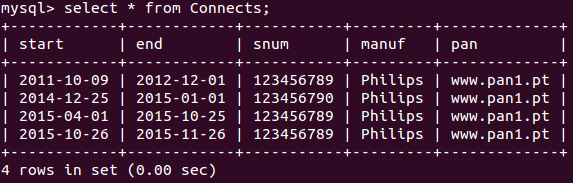
\includegraphics[scale=0.7]{tabelas_insert_triggers_Connects.png}
\caption{Tabela \textit{Connects}}
\end{figure}

\begin{figure}[ht!]
\centering
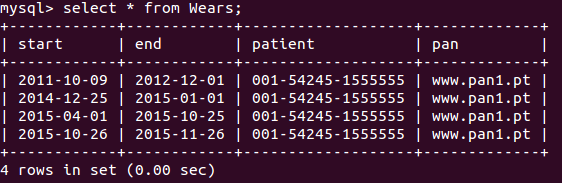
\includegraphics[scale=0.7]{tabelas_insert_triggers_Wears.png}
\caption{Tabela \textit{Wears}}
\end{figure}

\vskip 7mm
Os testes realizados foram sucessivas inserções de um dispositivo em PANs diferentes sobreposto a pelo menos uma entrada da tabela.

Os testes realizados estão contidos nos ficheiros \textit{teste\_insert\_connects.sql} e \textit{teste\_insert\_wears.sql}, apresentados em anexo e que contem uma série de instruções e respetivos comentários.

Correndo os ficheiros de teste verifica-se um de quatro dos seguintes resultados, consoante as tabelas a alterar e cosoante seja uma um \textit{update}/inserção válido ou inválido:

\begin{figure}[ht!]
\centering
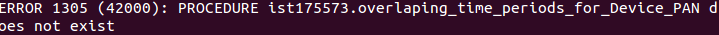
\includegraphics[scale=0.7]{erro_connect.png}
\caption{Mensagem de erro de inserção para a tabela \textit{Connects}}
\end{figure}

\begin{figure}[ht!]
\centering
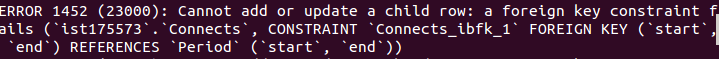
\includegraphics[scale=0.7]{good_connect.png}
\caption{Mensagem sucesso de inserção para a tabela \textit{Connects}}
\end{figure}

\begin{figure}[ht!]
\centering
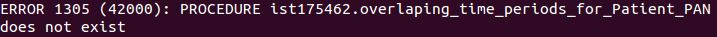
\includegraphics[scale=0.53]{error_wears.jpg}
\caption{Resultados dos testes do \textit{trigger} de inserção para a tabela \textit{Connects}}
\end{figure}

\begin{figure}[ht!]
\centering
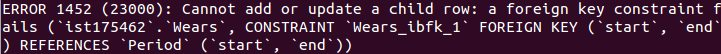
\includegraphics[scale=0.53]{good_wears.jpg}
\caption{Resultados dos testes do \textit{trigger} de inserção para a tabela \textit{Connects}}
\end{figure}

Em caso de sucesso, ou seja, sem sobreposição, surge uma mensagem de erro devido ao facto de o período inserido não existir na tabela \textit{Period}. Caso estivesse, não ocorreria o erro e a tabela seria atualizada.
\pagebreak
\subsection{\textit{Triggers} de \textit{update}}
À semelhança dos testes que realizámos para os \textit{triggers} de \textit{insert} para as duas tabelas, os ficheiros de teste para os \textit{triggers} de \textit{update} encontram-se em anexo, com os nomes \textit{teste\_update\_connects.sql} e \textit{teste\_update\_wears.sql}.

Os \textit{triggers} relativos a esta secção só diferem dos anteriores na medida em que são efetuados antes de um \textit{update} em vez de antes de um \textit{insert}. Assim, nos troços de código anteriores, onde se lê 

\textit{create trigger check\_overlap\_time\_period\_Patient\_PAN before insert on Wears} deve-se ler

 \textit{create trigger check\_overlap\_time\_period\_Patient\_PAN before update on Wears} e onde se lê
 
  \textit{create trigger check\_overlap\_time\_period\_Device\_PAN before insert on Connects} deve-se ler
  
   \textit{create trigger check\_overlap\_time\_period\_Device\_PAN before insert on Connects}.

No entanto, para esta secção foi utilizado um maior número de testes pois existe um maior número de casos de atualizações possíveis do que inserções.

Assim, a base de dados utilizada para os testes foi a presente no ficheiro \textit{database\_triggers\_update.sql}, sendo obtidas as seguintes tabelas:

\begin{figure}[ht!]
\centering
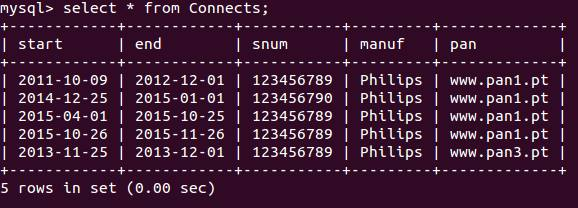
\includegraphics[scale=0.5]{update_connects.jpg}
\caption{Tabela \textit{Connects}}
\end{figure}

\begin{figure}[ht!]
\centering
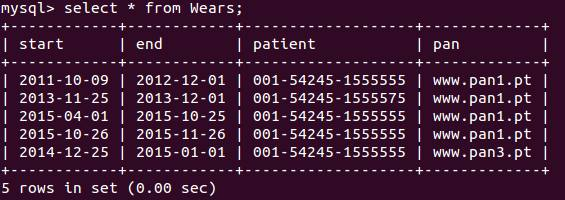
\includegraphics[scale=0.5]{update_wears.jpg}
\caption{Tabela \textit{Wears}}
\end{figure}


Na tabela da figura 7, a linha que é atualizada é sempre a última, correspondente a um \textit{device} igual a pelo menos um que se encontra na tabela. Porém, possui um PAN diferente destes.

Na tabela da figura 8, as linhas que são atualizadas são a segunda e última linhas que testam,  respetivamente, dois pacientes possuírem a mesma PAN simultaneamente e o mesmo paciente ter duas PANs simultaneamente.
\section{\textit{SQL queries}}
\subsection*{(a)}
A \textit{query} realizada para a alínea em questão foi a seguinte (presente no ficheiro \textit{3a.sql}):

\lstinputlisting{3a.sql}

Para testar o bom funcionamento do \textit{procedure}, utilizámos a base de dados presente em \textit{database3a.sql}, com o ficheiro de teste \textit{teste3a.sql}.

As tabelas obtidas deverão ser as seguintes:

\begin{figure}[ht!]
\centering
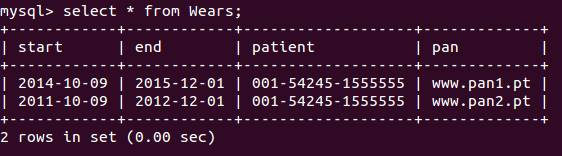
\includegraphics[scale=0.53]{3awears.jpg}
\caption{Tabela \textit{Wears}}
\end{figure}

\begin{figure}[ht!]
\centering
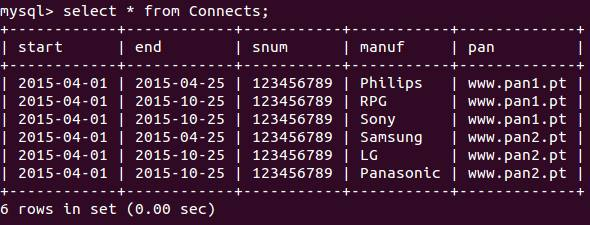
\includegraphics[scale=0.53]{3aconnects.jpg}
\caption{Tabela \textit{Connects}}
\end{figure}

\begin{figure}[ht!]
\centering
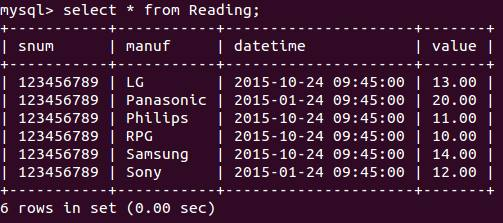
\includegraphics[scale=0.53]{3areading.jpg}
\caption{Tabela \textit{Reading}}
\end{figure}

\begin{figure}[ht!]
\centering
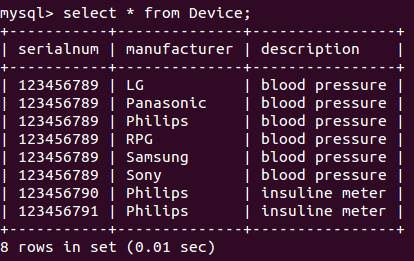
\includegraphics[scale=0.53]{3adevice.jpg}
\caption{Tabela \textit{Device}}
\end{figure}

Foram criados seis \textit{devices} de diferentes marcas, sendo que metade (RPG, Philips, Sony) foram associados à PAN cujo domínio é \textit{www.pan1.pt} e a restante (LG, Samsung, Panasonic) é colocada no PAN cujo domínio é \textit{www.pan2.pt}. Apenas um paciente, identificado pelo número 001-54245-1555555 irá conectar-se a estas PANs em dois períodos de tempo diferentes.
\vskip 16mm
Para o teste referido o resultado obtido será o seguinte:

\begin{figure}[ht!]
\centering
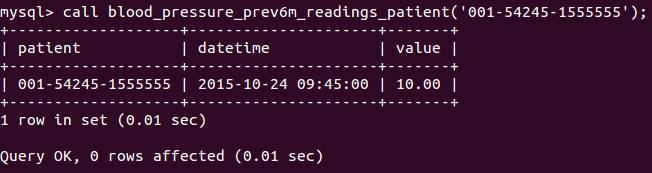
\includegraphics[scale=0.53]{teste3a.jpg}
\caption{Resultado do teste da \textit{query} 3 (a)}
\end{figure}

A explicação deste resultado, pode-se resumir em três pontos:

\begin{enumerate}
\item O Reading de RPG encontra-se dentro do período da data atual até 
	menos 6 meses, Philips também mas Sony não. Por outro lado no PAN2
	o Reading de LG encontra-se dentro do período da data actual até 
	menos 6 meses, Samsung também, mas Panasonic não;
\item O Reading de RPG encontra-se no período em que o Device está 
	conectado ao PAN1, mas o Reading de Philips não. No PAN2 o Reading
	de LG encontra-se dentro do período em que o Device está conectado  
	ao PAN2, mas o Reading de Samsung não;
\item O Reading de RPG encontra-se no período em que o Patient veste o
	PAN1, mas o Reading de LG não se encontra no período em que o Patient
	veste o PAN2.
\end{enumerate}

Desta forma, o primeiro ponto exclui Sony e Panasonic, o segundo ponto exclui Philips e Samsung e o terceiro Ponto exclui LG, restando RPG. A \textit{reading} associada a este aparelho encontra-se apresentada na figura 13.

\subsection*{(b)}
A \textit{query} realizada para a alínea em questão foi a seguinte (presente no ficheiro \textit{3b.sql}):

\lstinputlisting{3b.sql}

Para testar o bom funcionamento do \textit{procedure}, utilizámos a base de dados presente em \textit{database3b.sql}, com o ficheiro de teste \textit{teste3b.sql}.
\vskip 5mm
O resultado obtido deverá ser o seguinte:

\begin{figure}[ht!]
\centering
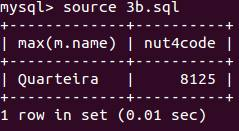
\includegraphics[scale=0.53]{3b.jpg}
\caption{Resultado do teste da \textit{query} 3 (b)}
\end{figure}

Para o teste em questão, foram criados nove Devices com manufacturer Philips com serial number
	diferentes mas consecutivos, três pacientes correspondentes aos elementos
	do grupo, três Municípios onde cada elemento viverá e quatro PANs.
	
	Para testar, fez-se com que o paciente Bernardo utilizasse duas PANS: PAN1
	e PAN2. O paciente Diogo utilizasse a PAN3 e o paciente Proença utilizasse a PAN4.
	
	A PAN1 possui três \textit{Devices}, PAN2 apenas um, PAN3 dois, e por
	fim PAN4 três \textit{Devices}, tendo todos os dispositivos descrições diferentes.
	
	Os \textit{Patients} Bernardo e Diogo vivem em Quarteira e Alcochete respetivamente num período que abrange a data atual, enquanto que o \textit{Patient}.
	Proença vive no Montijo num período que não abrange a data atual.
	
	Dos quatro \textit{Devices} que se encontram nos dois PANs que Bernardo utiliza, apenas
	três cumprem as especificações todas. Bernardo utiliza o PAN1 numa data 
	onde a data atual se encontra contida porém tal não acontece com PAN2,
	utilizando este PAN num período que não inclui a data atual.
	
	Todos os \textit{Devices} que se encontram nas Pans de Diogo e de Proença
	cumprem todas as especificações de tempo tanto de \textit{Wears} como \textit{Connects}
	em relação à data atual.
	
	Como Bernardo possui três \textit{Devices} que cumprem todas as especificações
	vence perante Diogo uma vez que este possui apenas dois.
	
	Como Bernardo vive num município numa data que abrange a atual vence
	perante Proença uma vez que este não cumpre esta condição.
	
	Assim o município que possui agora o maior número de \textit{Devices Philips}
	será Quarteira.
	
\subsection*{(c)}
A \textit{query} realizada para a alínea em questão foi a seguinte (presente no ficheiro \textit{3c.sql}):

\lstinputlisting{3c.sql}

Para testar o bom funcionamento do \textit{procedure}, utilizámos a base de dados presente em \textit{database3c.sql}, com o ficheiro de teste \textit{teste3c.sql}.
O resultado obtido deverá ser o seguinte:

\begin{figure}[ht!]
\centering
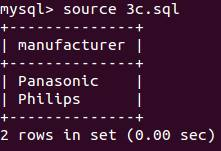
\includegraphics[scale=0.53]{teste3c.jpg}
\caption{Resultado do teste da \textit{query} 3 (c)}
\end{figure}

	Foram criados oito \textit{Devices} todos descritos por \textit{scale}, mas com \textit{serial
	number} e \textit{manufacturers} diferentes. Estes oito \textit{Devices} foram divididos
	por quatro \textit{Patients} correspondentes aos três elementos do grupo e o sem-abrigo
	Zé-Manel.
	
	O primeiro paciente Bernardo Gomes vive em Quarteira no ano de 2014,
	e utiliza o PAN1 durante os anos de 2013 e 2014, sendo que essa PAN 
	tem dois \textit{Devices (Philips e RPG)} conectados, um entre os anos 2013 e
	2014 e o outro no ano de 2015.
	
	O segundo paciente Diogo Martins vive em Alcochete no ano de 2014, e
	utiliza o PAN2 e PAN3 em duas alturas distintas, o primeiro entre 2014
	e 2015 e o segundo entre 2012 e 2013, sendo que o PAN2 possui um \textit{Device 
	(Panasonic)} ligado nos anos 2013 a 2015. O PAN3 tem também um dispositivo
	(\textit{LG}) ligado nos anos 2014 e 2014.
	
	O terceiro paciente Diogo Proença vive no Montijo entre 2011 e 2012,
	utilizando o PAN4 entre 2013 e 2014, sendo que o PAN4 possui dois \textit{Devices
	(Sony e Samsung)} associados, ambos ligados entre 2013 e 2014.
	
	O último paciente Zé Manel encontra-se de momento sem-abrigo, ou não
	vive em nenhum município presente na base de dados do \textit{Medical Center}.
	Porém utiliza o PAN5 entre 2013 e 2014 com dois \textit{Devices (Siemens e HP)}
	instalados nesse PAN entre 2013 e 2014.
	
	O resultado da Query será o apresentado na figura 15, com os seguintes dispositivos:
	
	\begin{itemize}
	\item \textit{Philips} $\rightarrow$ pois encontra-se conectado entre 2013 e 2014 num intervalo
	contido no período em que Bernardo utiliza o PAN durante o ano de 2014,
	acrescentado ao facto que Bernardo vive num município num intervalo
	também contido no período em que utiliza o PAN;
	
	\item \textit{Panasonic} $\rightarrow$ pois encontra-se conectado a PAN2 entre 2014 e 2015, num
	intervalo contido no período em que Diogo utiliza o PAN durante o ano 
	de 2014, acrescentado ao facto que Diogo vive num município num intervalo
	também contido no período em que utiliza o PAN.
	\end{itemize}
	
	Os dispositivos restantes apresentados de seguida, não cumprem as especificações pelas seguintes razões:
	
	\begin{itemize}
	\item \textit{RPG} $\rightarrow$ não cumpre a especificação de estar ligado ao PAN na mesma
	altura que Bernardo vive num município e utiliza essa PAN durante o ano de 2014.
	
	\item \textit{LG} $\rightarrow$ não cumpre a especificação de Diogo utilizar a PAN durante
	o ano de 2014 simultaneamente quando vive num município em 2014 e ter
	\textit{Devices} ligados à PAN.
	
	\item \textit{Sony e Samsung} $\rightarrow$ não cumprem a especificação de Proença estar
	a viver num município durante um ano de 2014 simultaneamente a estar
	a utilizar uma PAN e essa PAN ter tais \textit{Devices} ligados.
	
	\item \textit{Siemens e HP} $\rightarrow$ não cumprem a especificação pois Zé Manel não
	se encontra a viver num município coberto pelo Medical Center.
	\end{itemize}		
	
\section{\textit{Web based application}}
Para a aplicação \textit{web}, foi criada uma página inicial,

\textit{http://web.ist.utl.pt/ist175573/index\_\_.php} por forma a que o utilizador possa escolher quais as leituras e/ou alterações que pretende implementar na base de dados.
 
Assim, tal como pode ser verificado na figura 16, é feita uma distinção para ações de consulta da base de dados e de alterações à mesma. Tendo o trabalho apenas um fim académico, não foram implementadas todas as funcionalidades que seriam de esperar numa base de dados a apresentar a um cliente. Como tal, as funcionalidades dispostas são apenas as pedidas nas alíneas a) e b) do ponto quatro do enunciado do problema.

\begin{figure}[ht!]
\centering
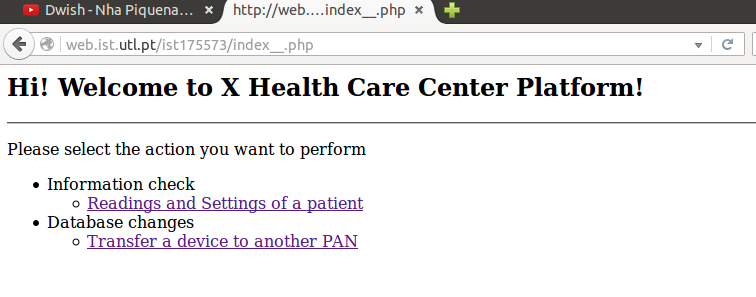
\includegraphics[scale=0.53]{index_php.png}
\caption{Página de apresentação da aplicação \textit{web}}
\end{figure}
	
No ponto a), pede-se que dado um certo paciente, sejam dispostos todos os seus dados de \textit{readings} e \textit{settings}. O utilizador poderá assim aceder a esta funcionalidade pela hiperligação \textit{Readings and Settings of a patient} do conjunto \textit{Information check}.

Ao fazê-lo, será redirecionado para uma página de formulário denominada \textit{Readings\_Settings.html} que pede o nome do paciente que se pretende saber as informações. Esta página encontra-se disposta na figura 17.

O resultado obtido no formulário passará posteriormente por uma página \textit{Patient\_intermidiate.php} com a finalidade de desambiguação. Assim, esta página, irá procurar todos os pacientes cujos nomes contenham a sequência de caracteres dadas pelo utilizador, questionando o mesmo qual dos pacientes é que se pretende obter os resultados.

No caso de o utilizador não escrever nenhuma sequência de caracteres, são apresentados todos os pacientes presentes na base de dados, tal como apresentado na figura 18.

\begin{figure}[ht!]
\centering
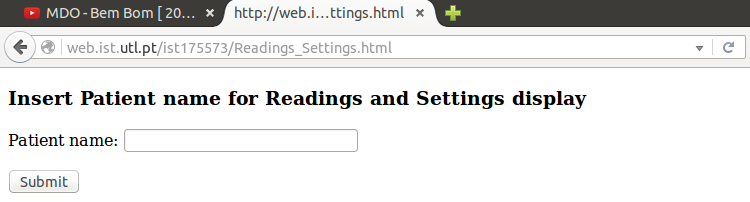
\includegraphics[scale=0.53]{Readings_Settings_html.png}
\caption{Página de recolha do nome do paciente}
\end{figure}

\begin{figure}[ht!]
\centering
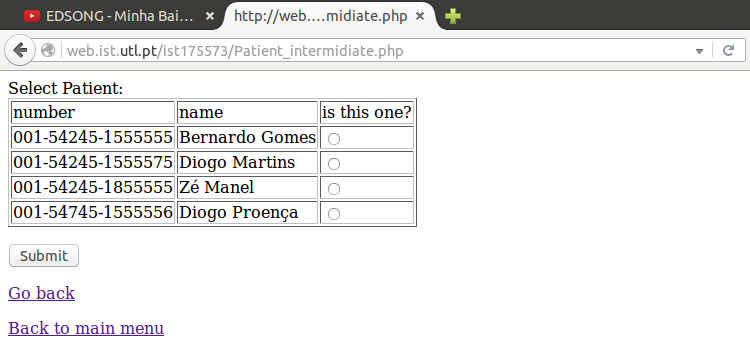
\includegraphics[scale=0.53]{Patient_intermidiate_php.png}
\caption{Página de desambiguação do nome do paciente}
\end{figure}

Este segundo \textit{form}, permite assim que o ficheiro seguinte saiba qual o SSN do paciente que o utilizador pretende, pelo que será dada a informação apenas de um paciente.

Após a recolha de informação deste formulário, o utilizador é direcionado para a página final \textit{Patient.php} que irá apresentar a informação pretendida. No caso de o paciente não ter registos associados, é disposta a informação que indica este facto.

São apresentadas de seguida os casos em que existe registos nas duas informações e em que não existe informação a apresentar.

\begin{figure}[ht!]
\centering
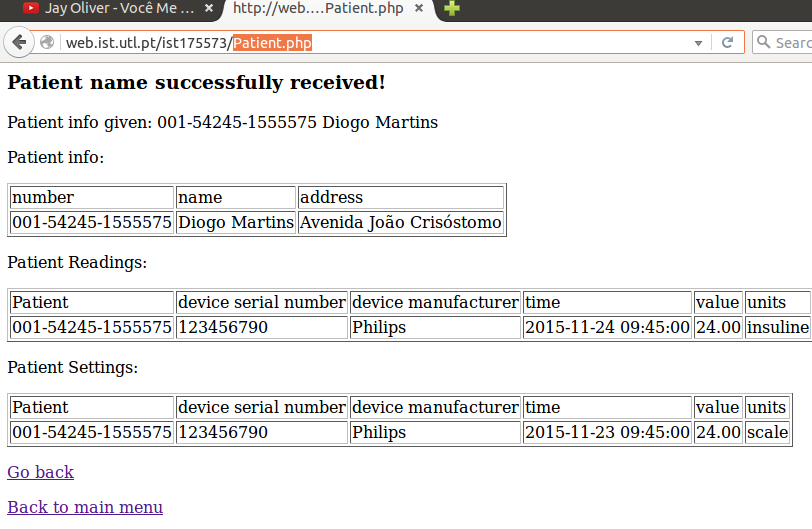
\includegraphics[scale=0.53]{diogo.png}
\caption{Apresentação dos \textit{Readings} e \textit{Settings}}
\end{figure}

\begin{figure}[ht!]
\centering
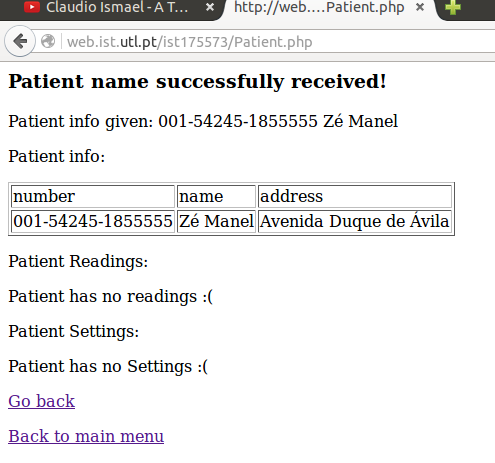
\includegraphics[scale=0.53]{ze.png}
\caption{Apresentação vazia dos \textit{Readings} e \textit{Settings}}
\end{figure}

\pagebreak
Seguindo a mesma lógica para a alínea (b), é feito o pedido do nome do paciente do qual se pretende fazer as transferências de \textit{devices} entre a PAN atual e a antiga, nos ficheiros \textit{Transfer\_device.html} e \textit{transfer\_intermediate.php}. A interface destas páginas é em tudo semelhante às apresentadas nas figuras 17 e 18, mudando apenas os títulos, pelo que não serão acrescentadas. Tendo o paciente sido escolhido, é apresentada a página \textit{transfer.php}, apresentada na figura 21, onde se pode visualizar todas as PANs associadas ao paciente, sendo especificada a PAN actual e a antiga mais recente.

\begin{figure}[ht!]
\centering
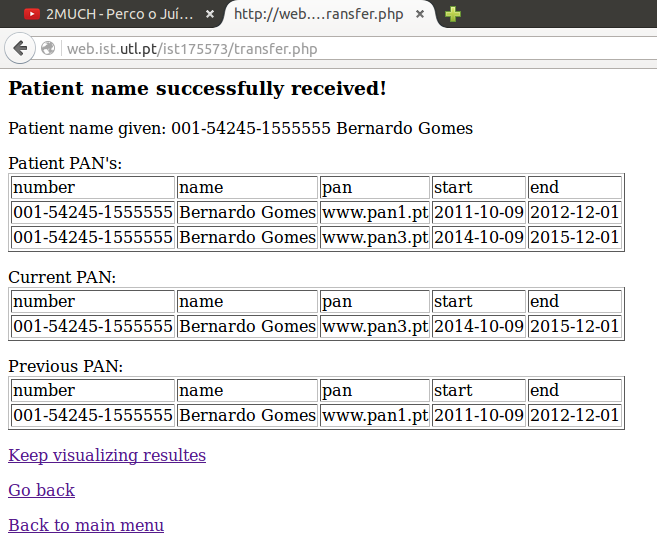
\includegraphics[scale=0.53]{transfer_php.png}
\caption{Apresentação vazia dos \textit{Readings} e \textit{Settings}}
\end{figure}
\vskip 9mm
Ao seguir o \textit{link} \textit{Keep visualizing resultes}, a página \textit{transfer\_session2.php} irá apresentar os aparelhos ligados a ambas as PANs, tendo uma interface incorporada que permite escolher via \textit{checkboxes} quais os aparelhos que se pretende transferir da PAN antiga para a actual. No caso de a PAN antiga estar a ser utilizada, ou de os aparelhos já terem sido transferidos, as \textit{checkboxes} não serão apresentadas, pelo que não se realizará a transferência desse dispositivo.

\begin{figure}[ht!]
\centering
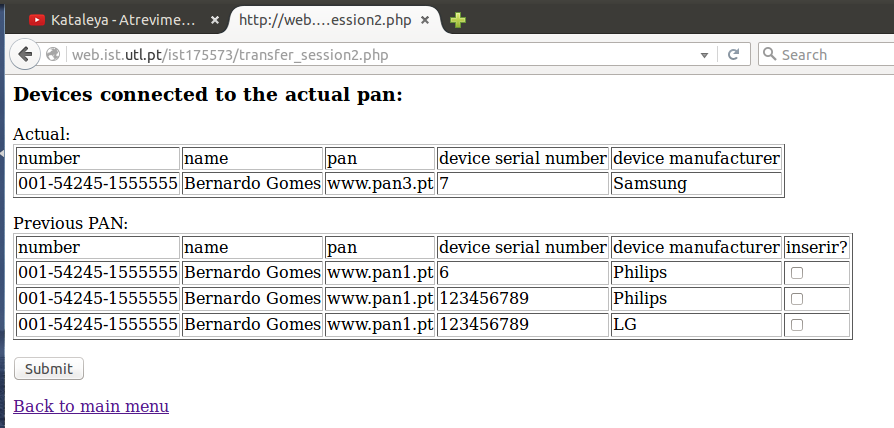
\includegraphics[scale=0.3]{transfer2.png}
\caption{Apresentação dos dispositivos e interface de transferência}
\end{figure}

Por fim, após a transferência dos \textit{devices} pretendidos, aparecerá uma página \textit{transfer\_session3.php} que indicará se a transferência foi bem sucedida e quais os dispositivos transferidos.

 \begin{figure}[ht!]
\centering
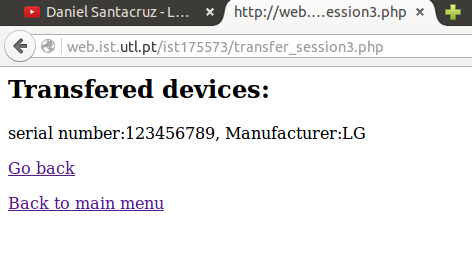
\includegraphics[scale=0.53]{transfer3.png}
\caption{Apresentação dos dispositivos transferidos}
\end{figure}

Caso se pressione \textit{Go back}, aparecerá novamente a interface de transferência, sendo que é visível a impossibilidade de inserir novamente o dispositivo.

 \begin{figure}[ht!]
\centering
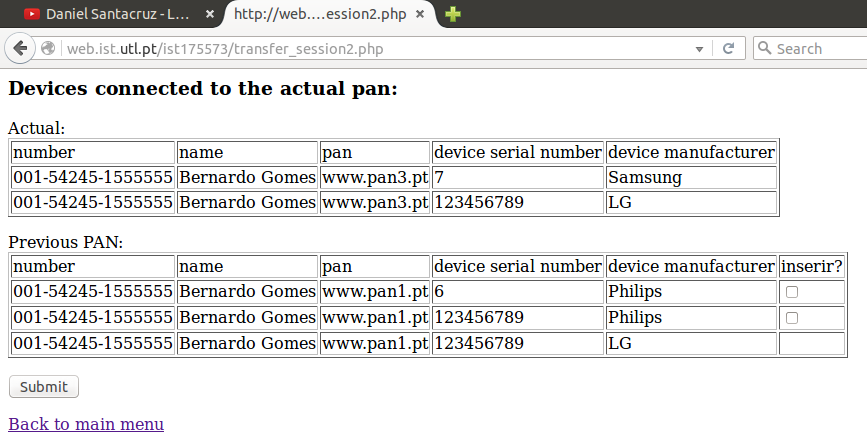
\includegraphics[scale=0.4]{transfer4.png}
\caption{Apresentação dos dispositivos transferidos, após LG ter sido transferido}
\end{figure}

Na maioria das páginas, é dada a possibilidade de voltar à página anterior bem como ao menu inicial.
\vskip 9mm
No caso de as imagens apresentadas no relatório não coincidirem com as tentativas, significará que a base de dados foi modificada.
\pagebreak
\section{Anexos}
Nesta secção são apresentados os códigos php, html e sql utilizados em cada secção.
\end{document}